\section{Visualising the data}
\paragraph{}
Let us first look at our data.
We're working with 2D data, so we can consider them as points.
There are $300$ points in the training data set, as well as $300$ points in the data set.
All of these points are \emph{labeled}, so we are dealing with a \emph{supervised classification} problem.
We have 3 classes and each class has $100$ points in each dataset.

\paragraph{}
In the figure below, we can see how the points are arranged.
Each color stands for a class, and the \emph{mean point} for each class was drawn using a filled circle.

\begin{figure}[H]
    \centering
    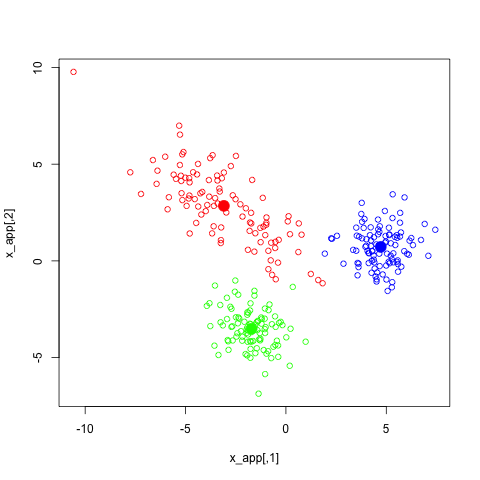
\includegraphics[width=\textwidth/2 - 5pt]{train_data.png}
    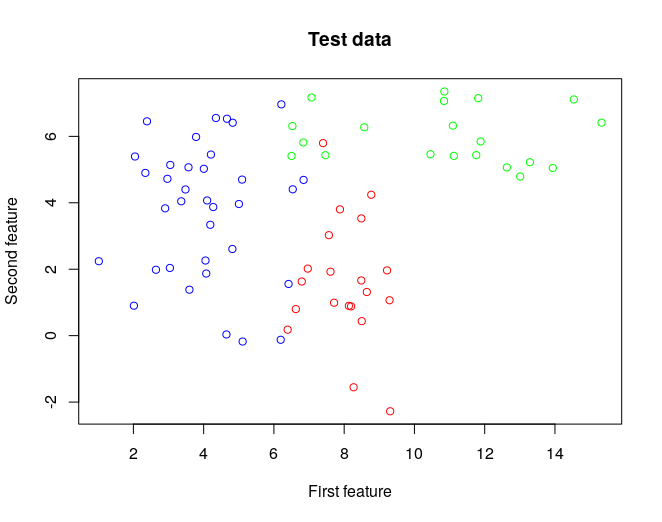
\includegraphics[width=\textwidth/2 - 5pt]{test_data.png}
    \caption{Train data on the left, test data on the right}
    \label{figure:data}
\end{figure}

\paragraph{}
Visualising the figures, we see that the points are similarily dispersed.
The red points (class 1) go from the upper left to the middle, the green points (class 2) tend to be in the middle-bottom and the blue ones (class 3) tend to be in the middle-right.
It also seems that the points in the test dataset are more scattered, while in the train dataset they tend to have a stronger ``cohesion''.
As a result, it seems easier to draw decision boundaries for the train dataset, but overall they aren't very hard to separate.

\clearpage

\section{Principal Component Analysis}

\subsection{Finding the best component}
\paragraph{}
We'll use PCA to find the best axis to project our data from.
That should be the one that allows the data to best be separated, or equally said, \emph{discriminated}.
To find that, we'll calculate the \emph{covariance matrix}, afterwards we'll choose the \emph{eigen vector} corresponding to the highest \emph{eigen value} for the covariance matrix.

\begin{lstlisting}[language=R, caption=Calculating the most discriminating axis]
# calculate covariance
covariance <- cov(x_app)
# get the eigen vectors and values
Vp <- eigen(covariance)
pente <- Vp$vectors[2, 1] / Vp$vectors[1, 1]
# visualise the best axis to project the data on
plot (x_app, col = trainColors)
abline(a = 0, b = pente, col = "orange")
\end{lstlisting}

\paragraph{}
Having this, we can now \emph{project} our training data on the axis:

\begin{lstlisting}[language=R, caption=Calculating the most discriminating axis]
ScalarProduct_app_ACP <- x_app %*% (Vp$vectors[, 1]) / sqrt(sum(Vp$vectors[, 1] * Vp$vectors[, 1]))
appProjections <- array(dim = dim(x_app))
appProjections[, 1] <- ScalarProduct_app_ACP * Vp$vectors[1, 1]
appProjections[, 2] <- ScalarProduct_app_ACP * Vp$vectors[2, 1]
\end{lstlisting}

\begin{figure}[!h]
    \centering
    \hspace{-1cm}%
    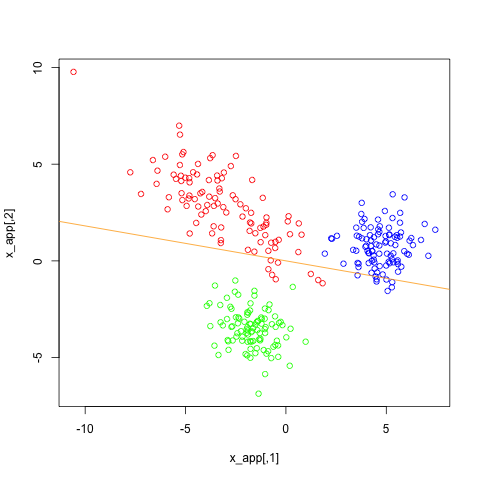
\includegraphics[width=\textwidth/2 - 5pt]{projection_line_acp.png}
    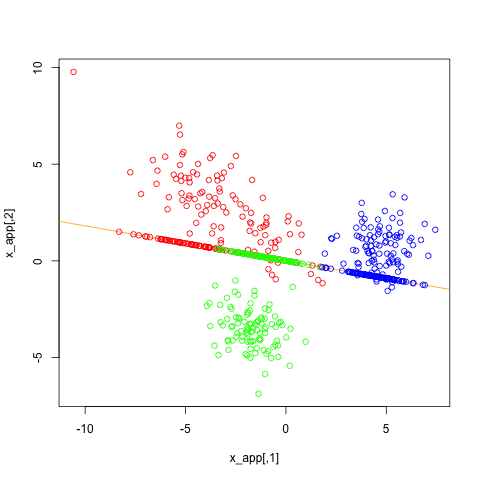
\includegraphics[width=\textwidth/2 - 5pt]{train_projections_acp.png}
    
    \begin{minipage}[t]{.5\textwidth}
    \centering
    \subcaption{Best axis according to PCA}
    \end{minipage}
    
    \begin{minipage}[t]{.5\textwidth}
    \centering
    \subcaption{Train data projected on the axis}
    \end{minipage}
\end{figure}


\paragraph{}
If we were to separate the training data based on their projections, we wouldn't have much luck.
Separating the blue class from the others doesn't pose a big problem, but the red and green classes overlap each other in a big proportion.


\clearpage

\subsection{Classifying data using PCA and LDA}
\paragraph{}
We can now use Linear Discriminant Analysis to predict our data, in combination with PCA.
We'll just train the LDA on the scalar products calculated above, as those resulted from PCA reducing our problem's dimensionality.
But before moving on, let's see how the test dataset looks like when it's projected on the axis we calculated:

\begin{figure}[H]
    \centering
    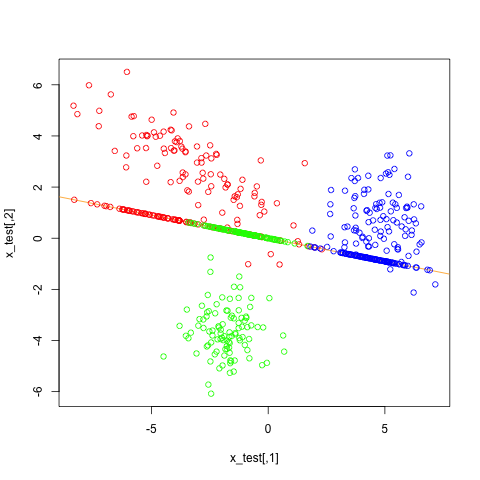
\includegraphics[width=\textwidth*2/3]{test_projections_acp.png}
    \caption{Test data projected on the PCA axis}
    \label{figure:test-projections}
\end{figure}

\paragraph{}
We can see that the same thing happens for the test data.
The red class overlaps the green class in a big proportion, so we can expect the test instances from the red class to not be properly predicted.
This is the script that calculates the predictions, based on the results from PCA:

\begin{lstlisting}[language=R, caption=Training LDA with PCA]
ScalarProduct_test_ACP <- x_test %*% (Vp$vectors[, 1]) / sqrt(sum(Vp$vectors[, 1] * Vp$vectors[, 1]))
x_app_ACP.lda <- lda(ScalarProduct_app_ACP, classe_app)
assigne_test <- predict(x_app_ACP.lda,  newdata = ScalarProduct_test_ACP)
\end{lstlisting}

\clearpage

\paragraph{}
Below we can see the results of the prediction.
In the figure below \ref{figure:test-predictions-lda-pca} and the following figures that contain predictions, for each point, the color represents its true class, and the shape represents our prediction.
Therefore, correct predictions are: red squares, green circles and blue triangles.
Anything else represents an error, a missclassification.

\begin{figure}[H]
    \centering
    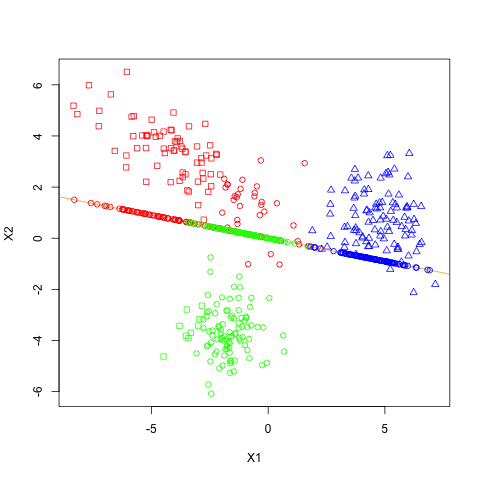
\includegraphics[width=\textwidth*2/3]{test_predictions_lda_acp.png}
    \caption{Test predictions, LDA with PCA}
    \label{figure:test-predictions-lda-pca}
\end{figure}

\paragraph{}
As we concluded from the figure above \ref{figure:test-projections}, we got a bad accuracy for the red points: only $69\%$ of them were classified correctly, because of the overlapping.
For the green class, the result is satisfying.
The blue class even has $100\%$ accuracy, since the blue projections can easily be separated from the rest.

\begin{center}
    \begin{tabular}{ |c|c|c|c|c| }
        \hline
        Method name & Red accuracy & Green accuracy & Blue accuracy & Total accuracy \\
        \hline
        LDA\&PCA & $69\%$ & $91\%$ & $100\%$ & $\approx 87\%$ \\
        \hline
    \end{tabular}
\end{center}

\clearpage

\section{Factorial Discriminant Analysis}

\subsection{Finding the most discriminating axis}
\paragraph{}
As \cite{dimensionality_reduction} states, in order to find the most discriminating axis using Factorial Analysis, we first need need some pre-calculations.
Having the means shown in the first figures \ref{figure:data}, we can calculate \emph{intra-class} co-variance and \emph{inter-class} co-variance.
We then apply the same method of finding the ``best'' eigen vector for the intra-class co-variance matrix.

\begin{lstlisting}[language=R, caption=Finding best discriminant axis using FDA]
trainMeans = array(dim = c(noClasses, dim(x_app)[2]))
for (i in 1:noClasses){
    trainMeans[i, 1] = mean(x_app[classe_app == i, 1])
    trainMeans[i, 2] = mean(x_app[classe_app == i, 2])
}
mean = colMeans(trainMeans)
# calculate covariances
S1 <- cov(x_app[classe_app==1,])
S2 <- cov(x_app[classe_app==2,])
S3 <- cov(x_app[classe_app==3,])
# intra-class, inter-class covariances
Sw = S1 + S2 + S3
Sb <- 0
for (i in 1:3)
    Sb <- Sb + (trainMeans[i,] - mean) %*% t(trainMeans[i,] - mean)

invSw <- solve(Sw)
invSw_by_Sb <- invSw %*% Sb
Vp <- eigen(invSw_by_Sb)
\end{lstlisting}

\paragraph{}
Here's the axis found by FDA, along with the projections from the train dataset on that axis:

\begin{figure}[!h]
    \centering
    \hspace{-1cm}%
    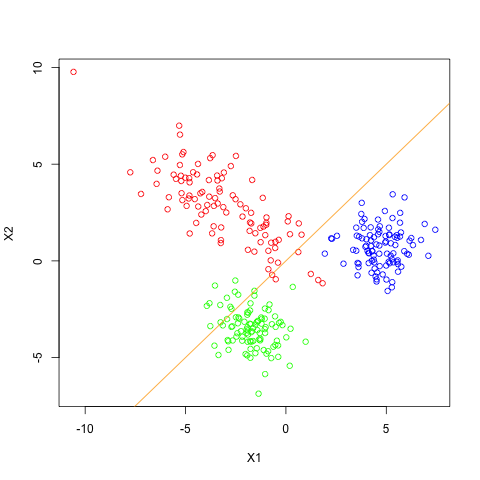
\includegraphics[width=\textwidth/2 - 5pt]{projection_line_afd.png}
    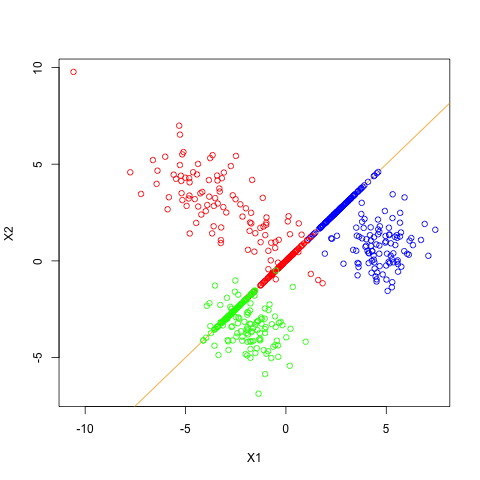
\includegraphics[width=\textwidth/2 - 5pt]{train_projections_afd.png}
    
    \begin{minipage}[t]{.5\textwidth}
    \centering
    \subcaption{Best axis according to FDA}
    \end{minipage}
    
    \begin{minipage}[t]{.5\textwidth}
    \centering
    \subcaption{Train data projected on the axis}
    \end{minipage}
\end{figure}

\paragraph{}
We can definitely see a big improvement.
The overlapping problem is much, much lower.
So, intuitively, we should expect better results if we were to combine FDA with LDA.

\clearpage

\subsection{LDA with FDA, comparison with PCA}
\paragraph{}
To classify our test data using AFD, we use the exact same code, but with the scalar products that resulted from FDA.
Here are the results:

\begin{figure}[H]
    \centering
    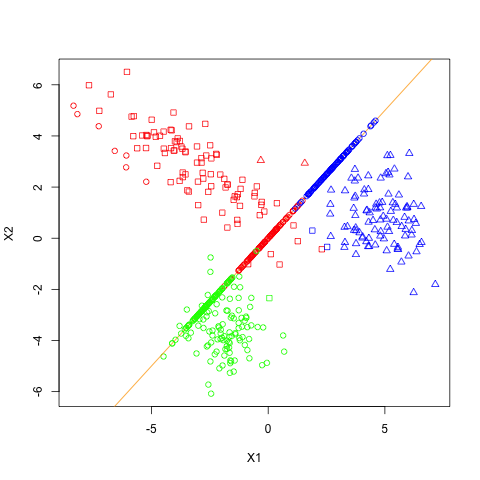
\includegraphics[width=\textwidth*2/3]{test_predictions_lda_afd.png}
    \caption{Test predictions, LDA with FDA}
\end{figure}

\begin{center}
    \begin{tabular}{ |c|c|c|c|c| }
        \hline
        Method name & Red accuracy & Green accuracy & Blue accuracy & Total accuracy \\
        \hline
        LDA\&PCA & $69\%$ & $91\%$ & $100\%$ & $\approx 87\%$ \\
        \hline
        LDA\&FDA & $91\%$ & $99\%$ & $98\%$ & $96\%$ \\
        \hline
    \end{tabular}
\end{center}

\paragraph{}
Comparing FDA with PCA, we have an improvement of $9\%$ on the total accuracy, which is a lot better.
This is mostly due to the fact that the red class is now classified much better, because we have a lot less overlapping.
The green instances have also seen a $7\%$ increase in accuracy, while we lost $2\%$ for the blue ones.
But, overall, it's much better.


\section{Training LDA directly on the training dataset}
\paragraph{}
For a final comparison, we can try to train the LDA directly on the training dataset.
The code is the same, we just train the LDA algorithm directly with our points: \lstinline[language=R]!x_app.lda <- lda(x_app, classe_app)!.

\begin{figure}[H]
    \centering
    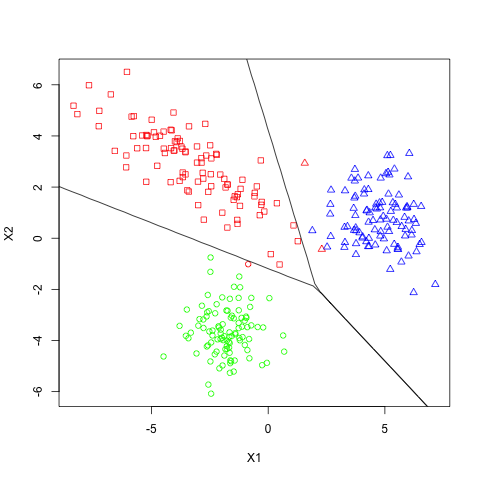
\includegraphics[width=\textwidth*2/3]{test_predictions_lda_contours.png}
    \caption{Test predictions, LDA trained directly on the training dataset}
\end{figure}

\paragraph{}
The figure above shows the decision boundaries for the LDA algorithm.
Here are the results:

\begin{center}
    \begin{tabular}{ |c|c|c|c|c| }
        \hline
        Method name & Red accuracy & Green accuracy & Blue accuracy & Total accuracy \\
        \hline
        LDA\&PCA & $69\%$ & $91\%$ & $100\%$ & $\approx 87\%$ \\
        \hline
        LDA\&FDA & $91\%$ & $99\%$ & $98\%$ & $96\%$ \\
        \hline
        LDA\&original data & $97\%$ & $100\%$ & $100\%$ & $99\%$ \\
        \hline
    \end{tabular}
\end{center}

\paragraph{}
There's a visible increase in accuracy, and that's normal.
Overall, LDA trained on the original data will give a total accuracy of $99\%$, which is really good.
It's normal – if the algorithm has more data to work with, it will provide better results.
But this is a trade-off that the decision-maker must settle.
If we want our algorithm to be faster, or to avoid the \emph{curse of dimensionality}, we should reduce the dimensionality of the problem (using, for example, PCA or AFD, like we did here), so the algorithm will train faster.
But, at the same time, it will most likely give less accurate results – however this is a question of overfit vs. underfit.